\documentclass{article}

\usepackage{graphicx}
\usepackage{tikz}
\usepackage{tikzsymbols}
\usetikzlibrary{calc,patterns,shapes.geometric}
\pagestyle{empty}
\usepackage[margin=0pt]{geometry}
\geometry{papersize={14in,12in}}

\def\centerarc[#1](#2)(#3:#4:#5){\draw[#1] ($(#2)+({#5*cos(#3)},{#5*sin(#3)})$) arc (#3:#4:#5);}

\begin{document}
	\begin{figure}
		\centering
		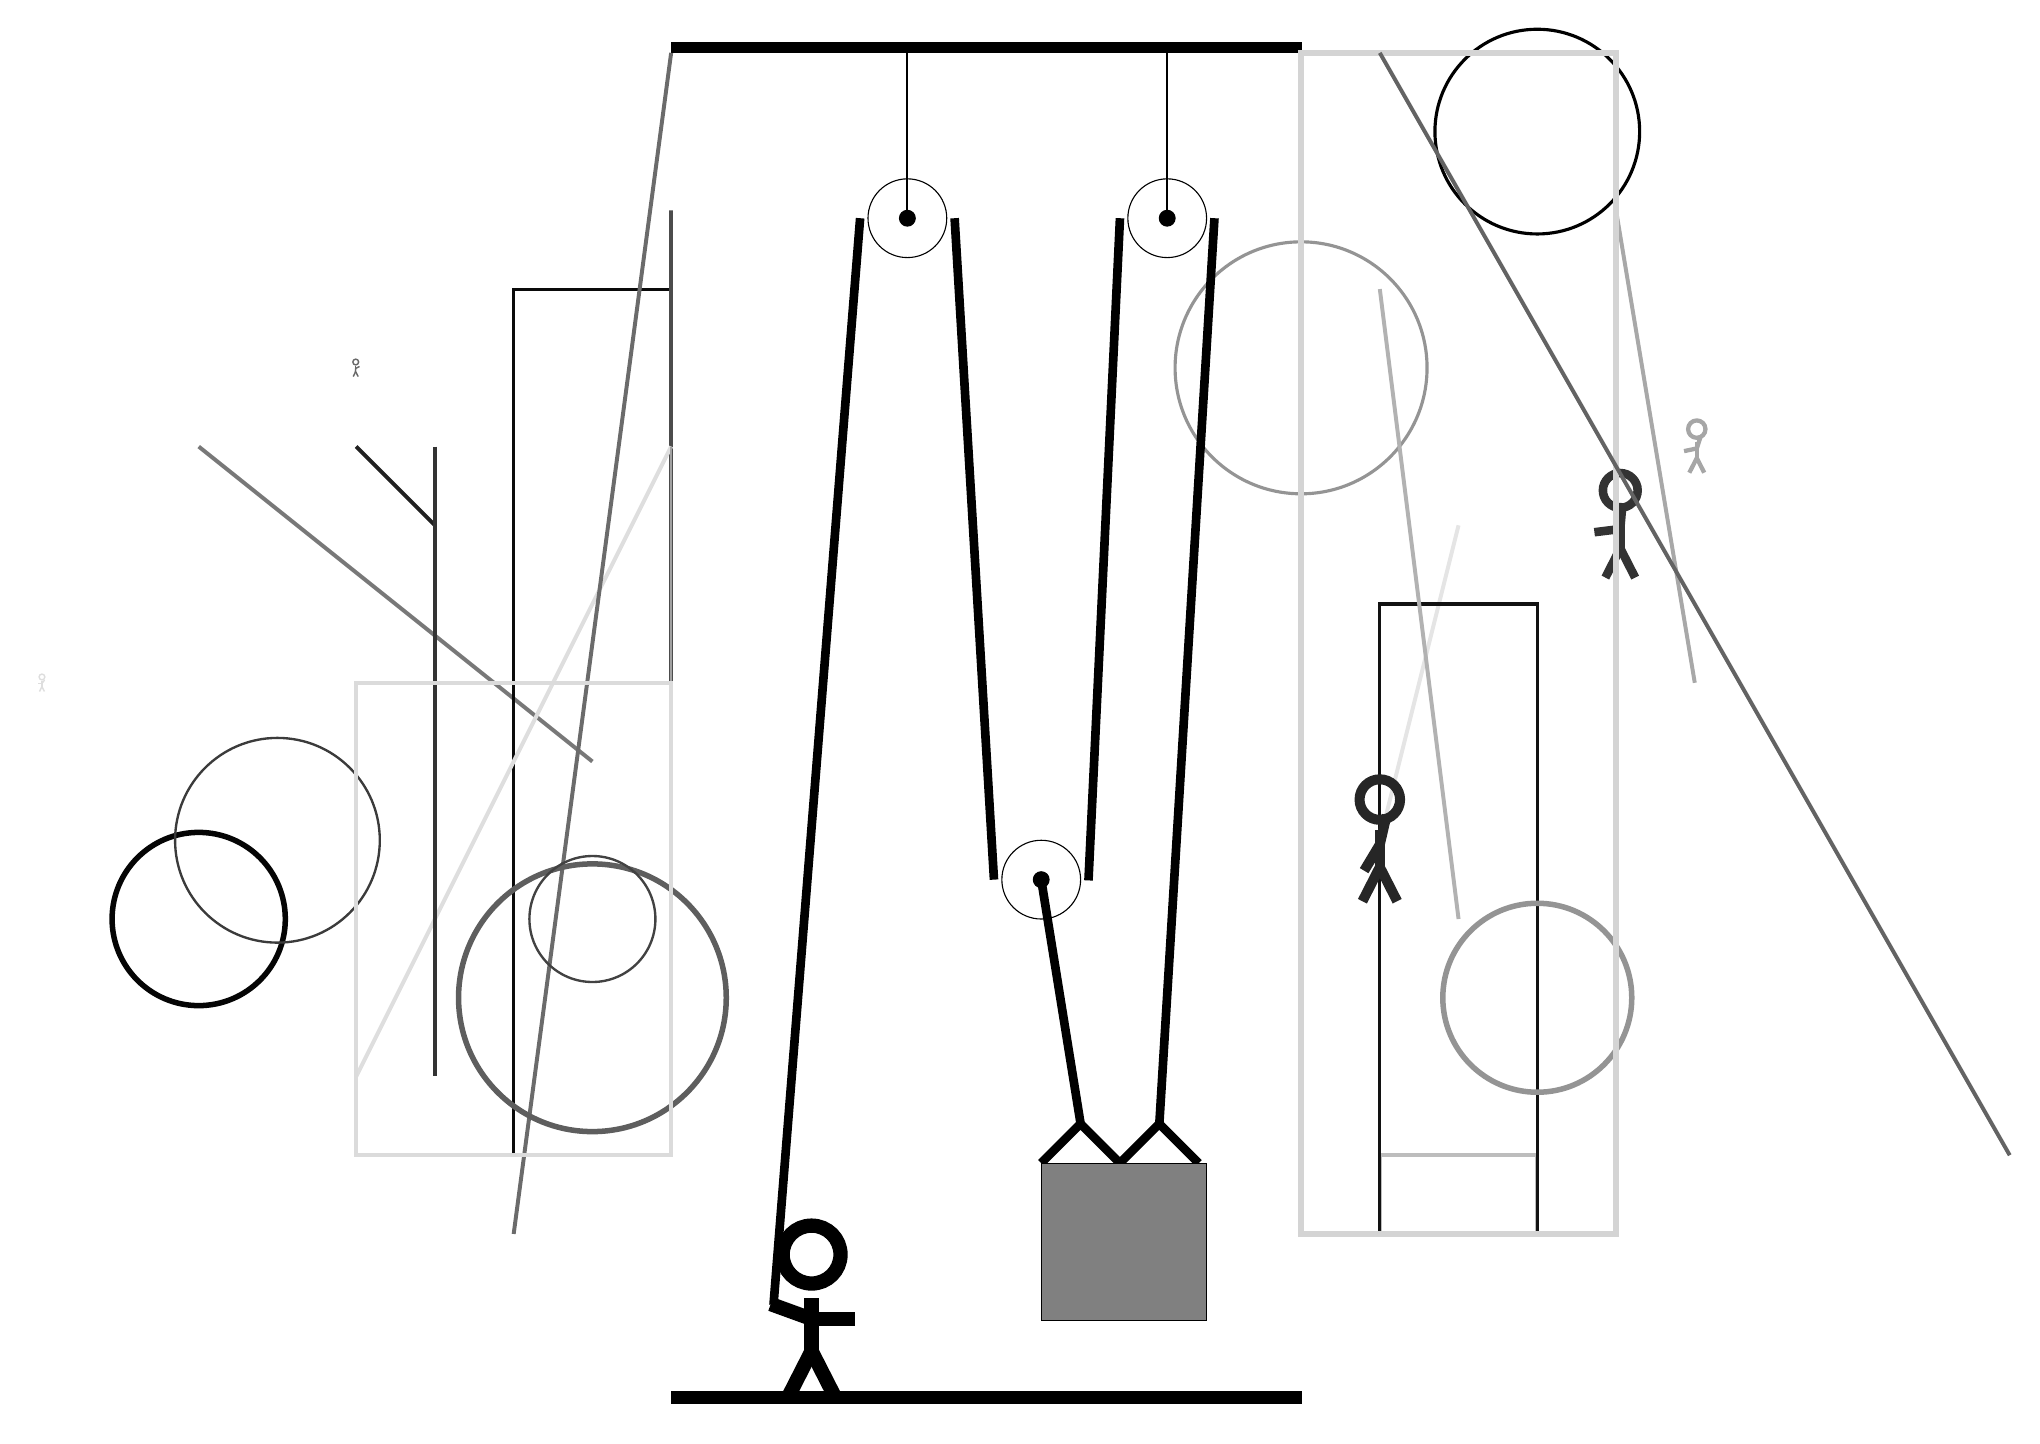
\begin{tikzpicture}
			%%%%% START %%%%%
			
			\draw[fill=black] (-2, 14) rectangle (6, 14.125);
			
			\draw (1, 11.9) circle (0.5);
			\draw[fill=black] (1, 11.9) circle (0.1);
			\draw[thick] (1, 11.9) -- (1, 14);
			
			\draw (4.3, 11.9) circle (0.5);
			\draw[fill=black] (4.3, 11.9) circle (0.1);
			\draw[thick] (4.3, 11.9) -- (4.3, 14);
			
			\draw (2.7, 3.5) circle (0.5);
			\draw[fill=black] (2.7, 3.5) circle (0.1);
			
			\draw[line width=1.1mm]  (2.7, -0.1) -- (3.2, 0.4) -- (3.7, -0.1) -- (4.2, 0.4) -- (4.7, -0.1);
			\draw[fill=black!50] (2.7, -0.1) rectangle (4.8, -2.1);
			
			\draw[line width=0.5mm, color=black!53](-3, 5) -- (-8, 9);
			
			\draw[line width=0.5mm, color=black!26] (7, -1) rectangle (9, 0);
			\draw [line width=0.7mm, color=black!98](-8, 3) circle (1.1);
			\draw[line width=0.5mm, color=black!10](7, 4) -- (8, 8);
			\draw[line width=0.4mm, color=black!96] (-4, 0) rectangle (-2, 11);
			\draw[line width=0.5mm, color=black!87](-5, 8) -- (-6, 9);
			\draw [line width=0.4mm, color=black!42](6, 10) circle (1.6);
			\draw[line width=0.4mm, color=black!93] (7, -1) rectangle (9, 7);
			\node[line width=0.7mm, color=black!80] at (10, 8) {\Strichmaxerl[6][7][85]};
			\draw[line width=0.5mm, color=black!70] (-2, 2) rectangle (-2, 12);
			\draw [line width=0.7mm, color=black!42](9, 2) circle (1.2);
			\draw[line width=0.5mm, color=black!13](-2, 9) -- (-6, 1);
			\draw[line width=0.2mm, color=black!37] (-2, 5) rectangle (-2, 9);
			
			\node[line width=0.4mm, color=black!13] at (-10, 6) {\Strichmaxerl[1][0][52]};
			\draw[line width=0.5mm, color=black!58](-2, 14) -- (-4, -1);
			\draw [line width=0.3mm, color=black!77](-7, 4) circle (1.3);
			
			\draw[line width=0.5mm, color=black!80](-5, 9) -- (-5, 1);
			\draw [line width=0.7mm, color=black!63](-3, 2) circle (1.7);
			\node[line width=0.6mm, color=black!35] at (11, 9) {\Strichmaxerl[3][12][72]};
			
			\node[line width=0.5mm, color=black!85] at (7, 4) {\Strichmaxerl[7][59][77]};
			\draw[line width=0.5mm, color=black!34](11, 6) -- (10, 12);
			
			\node[line width=0.5mm, color=black!59] at (-6, 10) {\Strichmaxerl[1][84][28]};
			\draw [line width=0.4mm, color=black!100](9, 13) circle (1.3);
			\draw[line width=0.3mm, color=black!62] (6, 6) rectangle (6, 7);
			\draw[line width=0.7mm, color=black!17] (6, 14) rectangle (10, -1);
			
			\draw[line width=0.5mm, color=black!30](8, 3) -- (7, 11);
			\draw[line width=0.5mm, color=black!14] (-2, 6) rectangle (-6, 0);
			\draw[line width=0.5mm, color=black!61](7, 14) -- (15, 0);
			
			\draw [line width=0.3mm, color=black!74](-3, 3) circle (0.8);
			
			
			\draw[line width=1.1mm](-0.7, -1.9) -- (0.4, 11.9);
			\centerarc[line width=1.1mm](1, 11.9)(0:180:0.6);
			\draw[line width=1.1mm](1.6, 11.9) -- (2.1, 3.5);
			\centerarc[line width=1.1mm](2.7, 3.5)(180:370:0.6);
			\draw[line width=1.1mm] (3.3, 3.49) -- (3.7, 11.9);
			\centerarc[line width=1.1mm](4.3, 11.9)(0:180:0.6);
			\draw[line width=1.1mm](4.2, 0.4) -- (4.9, 11.9);
			\draw[line width=1.1mm] (3.2, 0.4) -- (2.7, 3.5);
			
			\node at (-0.2, -2) {\Strichmaxerl[10][-20][0]};
			
			\draw[fill=black] (-2, -3) rectangle (6, -3.15);
			
			%%%%% END %%%%%
		\end{tikzpicture}
	\end{figure}	
\end{document}